% defer/hazptr.tex
% From an C++ Standards Committee meeting:  "Can I hazptr cheezeberger?"

\section{Hazard Pointers}
\label{sec:defer:Hazard Pointers}
%
\epigraph{If in doubt, turn it inside out.}{\emph{Zara Carpenter}}

동시적으로 수행되는 레퍼런스 카운팅에서의 문제를 해결하는 한가지 방법은
레퍼런스 카운터들을 뒤집어서 구현하는 것으로,
데이터 원소에 저장되어 있는 정수를 증가시키는 게 아니라, CPU 별 (또는 쓰레드별)
리스트에 그 데이터 원소로의 포인터를 저장해 두는 것입니다.
이런 리스트의 각 원소들은 \emph{해저드 포인터}~\cite{MagedMichael04a} 라고
불립니다.\footnote{
	그와 독립적으로 다른 사람들에 의해 개발된 것도
	있습니다~\cite{HerlihyLM02}.}
주어진 데이터 원소의 ``가상 레퍼런스 카운터'' 의 값은 그 원소를 레퍼런스 하고
있는 해저드 포인터들의 갯수를 세는 것으로 얻어질 수 있습니다.
따라서, 그 원소가 읽기를 하는 쓰레드들에 의해 접근할 수 없게 된다면, 그리고
더이상 그 원소를 레퍼런스 하고 있는 해저드 포인터가 더이상 존재하지 않는다면,
그 원소는 안전하게 메모리 해제될 수 있습니다.
\iffalse

One way of avoiding problems with concurrent reference counting
is to implement the reference counters
inside out, that is, rather than incrementing an integer stored in the
data element, instead store a pointer to that data element in
per-CPU (or per-thread) lists.
Each element of these lists is called a
\emph{hazard pointer}~\cite{MagedMichael04a}.\footnote{
	Also independently invented by others~\cite{HerlihyLM02}.}
The value of a given data element's ``virtual reference counter'' can
then be obtained by counting the number of hazard pointers referencing
that element.
Therefore, if that element has been rendered inaccessible to readers,
and there are no longer any hazard pointers referencing it, that element
may safely be freed.
\fi

\begin{listing}[tbp]
\input{CodeSamples/defer/hazptr@record_clear.fcv}
\caption{Hazard-Pointer Recording and Clearing}
\label{lst:defer:Hazard-Pointer Recording and Clearing}
\end{listing}

물론, 이 말은 해저드 포인터 획득은 동시의 삭제들에 의한 버그 (파멸의
경주-destructive race- 라고도 합니다)를 막기 위해 매우 조심스럽게 행해져야만
함을 의미합니다.
\iffalse

Of course, this means that hazard-pointer acquisition must be carried
out quite carefully in order to avoid destructive races with concurrent
deletion.
\fi
\begin{lineref}[ln:defer:hazptr:record_clear]
그런 한가지 구현이
Listing~\ref{lst:defer:Hazard-Pointer Recording and Clearing} 에 보여져 있는데,
line~\lnref{htr:b}-\lnref{htr:e} 에 \co{hp_try_record()} 를,
line~\lnref{hr:b}-\lnref{hr:e} 에 \co{hp_record()} 를, 그리고
line~\lnref{hc:b}-\lnref{hc:e} 에 \co{hp_clear()} 를 보이고 있습니다
(\path{hazptr.h}).
\iffalse

One implementation is shown in
Listing~\ref{lst:defer:Hazard-Pointer Recording and Clearing},
which shows \co{hp_try_record()} on lines~\lnref{htr:b}-\lnref{htr:e},
\co{hp_record()} on lines~\lnref{hr:b}-\lnref{hr:e}, and
\co{hp_clear()} on
lines~\lnref{hc:b}-\lnref{hc:e} (\path{hazptr.h}).
\fi

Line~\lnref{htr:e} 의 \co{hp_try_record()} 매크로는 단순히 \co{_h_t_r_impl()}
함수로의 캐스팅 wrapper 로, \co{p} 로 레퍼런스 되는 포인터를 \co{hp} 로
레퍼런스 되는 해저드 포인터 안에 저장하려 시도합니다.
이에 성공하면, 저장된 포인터의 값을 리턴합니다.
포인터가 \co{NULL} 이어서 실패한다면, \co{NULL} 을 리턴합니다.
마지막으로, 업데이트와의 경주상황으로 인해 실패한다면, \co{HAZPTR_POISON}
이라는 특수한 토큰을 리턴합니다.
\iffalse

The \co{hp_try_record()} macro on line~\lnref{htr:e} is simply a casting
wrapper for the \co{_h_t_r_impl()} function, which attempts to store
the pointer referenced by \co{p} into the hazard pointer referenced
by \co{hp}.
If successful, it returns the value of the stored pointer.
If it fails due to that pointer being \co{NULL}, it returns \co{NULL}.
Finally, if it fails due to racing with an update, it returns a special
\co{HAZPTR_POISON} token.
\fi

\QuickQuiz{}
	해저드 포인터들에 대한 논문들은 각각의 포인터의 아래 비트들을 지워진
	원소들을 마크하기 위해 사용한다고 하는데, \co{HAZPTR_POISON} 은 뭔가요?
	\iffalse

	Given that papers on hazard pointers use the bottom bits
	of each pointer to mark deleted elements, what is up with
	\co{HAZPTR_POISON}?
	\fi
\QuickQuizAnswer{
	출간된 논문의 해저드 포인터 구현들은 그 삽입과 삭제를 위해 non-blocking
	동기화 기법들을 사용했습니다.
	이런 기법들은 데이터 구조체를 가로지르며 읽기를 하는 쓰레드들이
	업데이트를 하는 쓰레드들이 그들의 업데이트를 완료하도록 ``도움''을 줄
	것을 필요로 하는데, 이 말은 읽기를 하는 쓰레드들은 삭제된 원소의 다음
	원소를 봐야만 한다는 뜻입니다.

	반면에, 우리는 업데이트 작업들을 동기화 시키는데 락킹을 사용할 것인데,
	이렇게 되면 읽기를 하는 쓰레드들이 업데이트를 하는 쓰레드들이 그들의
	업데이트를 완료할 수 있도록 돕는 일을 해줄 필요가 없어져서 포인터들의
	아래쪽 비트들을 놔둘 수 있게 해줍니다.
	이 방법은 읽기를 하는쪽 코드를 좀 더 간단하고 빠르게 해줍니다.
	\iffalse

	The published implementations of hazard pointers used
	non-blocking synchronization techniques for insertion
	and deletion.
	These techniques require that readers traversing the
	data structure ``help'' updaters complete their updates,
	which in turn means that readers need to look at the successor
	of a deleted element.

	In contrast, we will be using locking to synchronize updates,
	which does away with the need for readers to help updaters
	complete their updates, which in turn allows us to leave
	pointers' bottom bits alone.
	This approach allows read-side code to be simpler and faster.
	\fi
} \QuickQuizEnd

Line~\lnref{htr:ro1} 은 보호되야 하는 오브젝트로의 포인터를 읽습니다.
Line~\lnref{htr:race1} 이 이 포인터가 \co{NULL} 이거나 특수한 삭제된 오브젝트
토큰인 \co{HAZPTR_POISON} 이라면, 호출자에게 실패를 알리기 위해 이 포인터의
값을 리턴합니다.
그렇지 않다면, line~\lnref{htr:store} 는 명시된 해저드 포인터로의 포인터를
저장하고, line~\lnref{htr:mb} 에서 이 저장을 line~\lnref{htr:ro2} 에서의 원래
포인터의 다시 읽기와 완전히 순서맞춰질 것을 강제합니다.
(메모리 순서 규칙에 대한 더 많은 정보를 위해선
Chapter~\ref{chp:Advanced Synchronization: Memory Ordering} 를 참고하세요.)
원래 포인터의 값이 변하지 않았다면, 이 해저드 포인터는 가리켜진 오브젝트를
보호하며, 이 경우, line~\lnref{htr:success} 는 해당 오브젝트로의 포인터를
리턴하는데, 이는 호출자에게 성공을 의미하기도 합니다.
그렇지 않고, 포인터가 두개의 \co{READ_ONCE()} 호출 사이에 변했다면,
line~\lnref{htr:race2} 가 실패를 알립니다.

\iffalse
Line~\lnref{htr:ro1} reads the pointer to the object to be protected.
If line~\lnref{htr:race1} finds that this pointer was either \co{NULL} or
the special \co{HAZPTR_POISON} deleted-object token, it returns
the pointer's value to inform the caller of the failure.
Otherwise, line~\lnref{htr:store} stores the pointer into the specified
hazard pointer, and line~\lnref{htr:mb} forces full ordering of that
store with the reload of the original pointer on line~\lnref{htr:ro2}.
(See Chapter~\ref{chp:Advanced Synchronization: Memory Ordering}
for more information on memory ordering.)
If the value of the original pointer has not changed, then the hazard
pointer protects the pointed-to object, and in that case,
line~\lnref{htr:success} returns a pointer to that object, which also
indicates success to the caller.
Otherwise, if the pointer changed between the two \co{READ_ONCE()}
invocations, line~\lnref{htr:race2} indicates failure.
\fi

\QuickQuiz{}
	Listing~\ref{lst:defer:Hazard-Pointer Recording and Clearing}
	의 \co{hp_try_record()} 는 왜 데이터 원소로의 이중 간접 접근을
	취하나요?
	왜 \co{void *} 대신 \co{void **} 인가요?
	\iffalse

	Why does \co{hp_try_record()} in
	Listing~\ref{lst:defer:Hazard-Pointer Recording and Clearing}
	take a double indirection to the data element?
	Why not \co{void *} instead of \co{void **}?
	\fi
\QuickQuizAnswer{
	\co{hp_try_record()} 는 동시의 수정을 체크해야 하기 때문입니다.
	이 일을 하기 위해선, 해당 원소로의 포인터로의 포인터가 있어서 해당
	원소로의 포인터로의 수정을 체크할 수 있어야 합니다.
	\iffalse

	Because \co{hp_try_record()} must check for concurrent modifications.
	To do that job, it needs a pointer to a pointer to the element,
	so that it can check for a modification to the pointer to the
	element.
	\fi
} \QuickQuizEnd

이 \co{hp_record()} 함수는 상당히 직관적입니다: 리턴값이 \co{HAZPTR_POISON} 이
아닌 무언가일 때까지 반복적으로 \co{hp_try_record()} 를 호출합니다.
\iffalse

The \co{hp_record()} function is quite straightforward: It repeatedly
invokes \co{hp_try_record()} until the return value is something other
than \co{HAZPTR_POISON}.
\fi

\QuickQuiz{}
	왜 \co{hp_try_record()} 로 귀찮게 하죠?
	실패에 문제 없는 \co{hp_record()} 함수를 대신 사용하는게 어때요?
	\iffalse

	Why bother with \co{hp_try_record()}?
	Wouldn't it be easier to just use the failure-immune
	\co{hp_record()} function?
	\fi
\QuickQuizAnswer{
	어떤 면에선 그게 더 쉽겠지만, 앞으로 Pre-BSD 라우팅 예제에서 보게
	되겠지만, \co{hp_record()} 가 먹히지 않는 경우도 있습니다.
	\iffalse

	It might be easier in some sense, but as will be seen in the
	Pre-BSD routing example, there are situations for which
	\co{hp_record()} simply does not work.
	\fi
} \QuickQuizEnd

The \co{hp_clear()} function is even more straightforward, with
an \co{smp_mb()} to force full ordering between the caller's uses
of the object protected by the hazard pointer and the setting of
the hazard pointer to \co{NULL}.
\end{lineref}

\begin{listing}[tbp]
\input{CodeSamples/defer/hazptr@scan_free.fcv}
\caption{Hazard-Pointer Scanning and Freeing}
\label{lst:defer:Hazard-Pointer Scanning and Freeing}
\end{listing}

\begin{lineref}[ln:defer:hazptr:scan_free:free]
해저드 포인터로 보호되는 객체가 자신의 연결된 데이터 구조에서 제거되어서 미래의
해저드 포인터 읽기 쓰레드에게 접근될 수 없게 되었다면, 이 객체는
\co{hazptr_free_later()} 에 넘겨지는데, 이 함수는
Listing~\ref{lst:defer:Hazard-Pointer Scanning and Freeing}
(\path{hazptr.c}) 에 의 line~\lnref{b}-\lnref{e} 에 보여져 있습니다.
Line~\lnref{enq:b} 와~\lnref{enq:e} 는 이 객체를 쓰레드별 리스트 \co{rlist} 에
집어넣고 line~\lnref{count} 는 \co{rcount} 내의 객체 수를 셉니다.
만약 line~\lnref{check} 가 이제 충분히 많은 객체가 들어와 있음을 보게 되면,
line~\lnref{scan} 이 이것들 중 일부를 메모리 해제시키기 위해 \co{hazptr_scan()}
을 호출합니다.
\iffalse

Once a hazard-pointer-protected object has been removed from its
linked data structure, so that it is now inaccessible to future
hazard-pointer readers, it is passed to \co{hazptr_free_later()},
which is shown on lines~\lnref{b}-\lnref{e} of
Listing~\ref{lst:defer:Hazard-Pointer Scanning and Freeing}
(\path{hazptr.c}).
Lines~\lnref{enq:b} and~\lnref{enq:e}
enqueue the object on a per-thread list \co{rlist}
and line~\lnref{count} counts the object in \co{rcount}.
If line~\lnref{check} sees that a sufficiently large number of objects are now
queued, line~\lnref{scan} invokes \co{hazptr_scan()} to attempt to
free some of them.
\fi
\end{lineref}

\begin{lineref}[ln:defer:hazptr:scan_free:scan]
\co{hazptr_scan()} 함수가 이 리스트의 line~\lnref{b}-\lnref{e} 에 보여져
있습니다.
이 함수는 고정된 쓰레드 최대 갯수 (\co{NR_THREADS}) 와 쓰레드별 해저드 포인터의
최대 갯수 (\co{K}) 에 의존적인데, 이는 해저드 포인터들의 고정된 크기 배열이
사용될 수 있게 합니다.
어떤 쓰레드건 이 해저드 포인터들을 스캔해야 할 수 있으므로, 각 쓰레드는 자신의
배열을 유지하는데, 이는 쓰레드별 변수 \co{gplist} 에 의해 레퍼런스 됩니다.
Line~\lnref{check} 가 이 쓰레드가 아직 자신의 \co{gplist} 를 할당받지 않았음을
파악하게 되면, line~\lnref{alloc:b}-\lnref{alloc:e} 가 이 할당을 진행합니다.
Line~\lnref{mb1} 의 메모리 배리어는 모든 쓰레드가 이 쓰레드에 의한 모든 객체의
제거를 line~\lnref{loop:b}-\lnref{loop:e} 가 모든 해저드 포인터를 스캔하고 NULL
이 아닌 포인터들을 \co{plist} 배열에 저장하고 그 갯수를 \co{psize} 에 세기 전에
보게 될 것을 보장합니다.
Line~\lnref{mb2} 의 메모리 배리어는 해저드 포인터의 읽기가 모든 객체의 메모리
해제 전에 일어날 것을 보장합니다.
Line~\lnref{sort} 는 이제 이 배열을 정렬시켜서 아래에 설명할 바이너리 탐색이
가능하게 합니다.
\iffalse

The \co{hazptr_scan()} function is shown on lines~\lnref{b}-\lnref{e}
of the listing.
This function relies on a fixed maximum number of threads (\co{NR_THREADS})
and a fixed maximum number of hazard pointers per thread (\co{K}),
which allows a fixed-size array of hazard pointers to be used.
Because any thread might need to scan the hazard pointers, each thread
maintains its own array, which is referenced by the per-thread variable
\co{gplist}.
If line~\lnref{check} determines that this thread has not yet allocated its
\co{gplist}, lines~\lnref{alloc:b}-\lnref{alloc:e} carry out the allocation.
The memory barrier on line~\lnref{mb1} ensures that all threads see the
removal of all objects by this thread before
lines~\lnref{loop:b}-\lnref{loop:e} scan
all of the hazard pointers, accumulating non-NULL pointers into
the \co{plist} array and counting them in \co{psize}.
The memory barrier on line~\lnref{mb2} ensures that the reads of
the hazard pointers
happen before any objects are freed.
Line~\lnref{sort} then sorts this array to enable use of binary search below.
\fi

Line~\lnref{rem:b} 와~\lnref{rem:e} 는 이 쓰레드의 메모리 해제 되기 위한
오브젝트들의 리스트에서 모든 원소들을 제거하고, 그것들을 로컬 \co{tmplist} 에
위치시키며 line~\lnref{zero} 는 그 카운트를 0으로 만듭니다.
Line~\lnref{loop2:b}-\lnref{loop2:e} 의 루프의 각 패스는 앞으로 메모리 해제될
오브젝트들 각각을 처리합니다.
Line~\lnref{rem1st:b} 와~\lnref{rem1st:e} 는 이 첫번째 오브젝트를 \co{tmplist}
에서 제거하고, line~\lnref{chkhazp:b} 와~\lnref{chkhazp:e} 가 이 오브젝트를
보호하는 해저드 포인터가 있음을 파악하면, line~\lnref{back:b}-\lnref{back:e} 는
이걸 도로 \co{rlist} 에 위치시킵니다.
그렇지 않다면, line~\lnref{free} 가 이 오브젝트를 해제시킵니다.
\iffalse

Lines~\lnref{rem:b} and~\lnref{rem:e}
remove all elements from this thread's list of
to-be-freed objects, placing them on the local \co{tmplist}
and line~\lnref{zero} zeroes the count.
Each pass through the loop spanning
lines~\lnref{loop2:b}-\lnref{loop2:e} processes each
of the to-be-freed objects.
Lines~\lnref{rem1st:b} and~\lnref{rem1st:e}
remove the first object from \co{tmplist},
and if lines~\lnref{chkhazp:b} and~\lnref{chkhazp:e}
determine that there is a hazard pointer
protecting this object, lines~\lnref{back:b}-\lnref{back:e}
place it back onto \co{rlist}.
Otherwise, line~\lnref{free} frees the object.
\fi
\end{lineref}

\begin{listing}[tbp]
\input{CodeSamples/defer/route_hazptr@lookup.fcv}
\caption{Hazard-Pointer Pre-BSD Routing Table Lookup}
\label{lst:defer:Hazard-Pointer Pre-BSD Routing Table Lookup}
\end{listing}

Pre-BSD 라우팅 예제는 해저드 포인터를 사용할 수 있는데,
Figure~\ref{lst:defer:Hazard-Pointer Pre-BSD Routing Table Lookup}
에서 그런 데이터 구조들과 \co{route_lookup()} 을 보이고 있고,
Figure~\ref{lst:defer:Hazard-Pointer Pre-BSD Routing Table Add/Delete}
에서 \co{route_add()} 와 \co{route_del()} 을 보이고 있습니다
(\path{route_hazptr.c}).
레퍼런스 카운팅에서와 마찬가지로, 해저드 포인터 구현은
page~\pageref{lst:defer:Sequential Pre-BSD Routing Table} 의
Figure~\ref{lst:defer:Sequential Pre-BSD Routing Table} 에서 보인 순차적
알고리즘과 상당히 유사하므로 차이점만 이야기하겠습니다.
\iffalse

The Pre-BSD routing example can use hazard pointers as shown in
Listing~\ref{lst:defer:Hazard-Pointer Pre-BSD Routing Table Lookup}
for data structures and \co{route_lookup()}, and in
Listing~\ref{lst:defer:Hazard-Pointer Pre-BSD Routing Table Add/Delete}
for \co{route_add()} and \co{route_del()}
(\path{route_hazptr.c}).
As with reference counting, the hazard-pointers implementation
is quite similar to the sequential algorithm shown in
Listing~\ref{lst:defer:Sequential Pre-BSD Routing Table}
on
page~\pageref{lst:defer:Sequential Pre-BSD Routing Table},
so only differences will be discussed.
\fi

\begin{lineref}[ln:defer:route_hazptr:lookup]
Listing~\ref{lst:defer:Hazard-Pointer Pre-BSD Routing Table Lookup}
에서 시작해서, line~\lnref{hh} 는 해저드 포인터 메모리 해제를 지연시키는
오브젝트를 대기열에 넣는데 사용되는 \co{->hh} 필드를 보이며,
line~\lnref{re_freed} 는 메모리 해제 후 사용 버그를 발견하기 위해 사용되는
\co{->re_freed} 필드를 보이며, line~\lnref{tryrecord} 는 해저드 포인터를 얻기
위해 \co{hp_try_record()} 를 호출합니다.
리턴값이 \co{NULL} 이라면, line~\lnref{NULL} 은 발견되지 않았음 신호를
호출자에게 리턴합니다.
만약 \co{hp_try_record()} 호출이 삭제와 경주를 행했다면, line~\lnref{deleted}
는 line~\lnref{retry} 의 \co{retry} 로 되돌아가 리스트를 시작부터 다시
횡단합니다.
이 \co{do}-\co{while} 루프는 원하는 원소가 찾아졌을 때 끝납니다만, 만약 이
원소가 이미 메모리 해제되었다면, line~\lnref{abort} 가 프로그램을 종료시킵니다.
그렇지 않다면, 이 원소의 \co{->iface} 필드가 호출자에게 리턴됩니다.
\iffalse

Starting with
Listing~\ref{lst:defer:Hazard-Pointer Pre-BSD Routing Table Lookup},
line~\lnref{hh} shows the \co{->hh} field used to queue objects pending
hazard-pointer free,
line~\lnref{re_freed} shows the \co{->re_freed} field used to detect
use-after-free bugs, and line~\lnref{tryrecord} invokes
\co{hp_try_record()} to attempt to acquire a hazard pointer.
If the return value is \co{NULL}, line~\lnref{NULL} returns a not-found
indication to the caller.
If the call to \co{hp_try_record()} raced with deletion, line~\lnref{deleted}
branches back to line~\lnref{retry}'s \co{retry} to re-traverse the list
from the beginning.
The \co{do}-\co{while} loop falls through when the desired element is
located, but if this element has already been freed, line~\lnref{abort}
terminates the program.
Otherwise, the element's \co{->iface} field is returned to the caller.
\fi

Line~\lnref{tryrecord} 가 더 사용하기 쉬운 \co{hp_record()} 대신
\co{hp_try_record()} 를 호출해서, \co{hp_try_record()} 의 실패 시에
전체 탐색을 재시작 함을 알아 두시기 바랍니다.
그리고 그런 재시작은 정확성을 위해 분명 필요합니다.  이를 보기 위해, 원소~A, B,
그리고~C 를 가지고 있고 해저드 포인터로 보호되는 링크드 리스트가 다음 이벤트를
겪는다고 생각해 봅시다:
\iffalse

Note that line~\lnref{tryrecord} invokes \co{hp_try_record()} rather
than the easier-to-use \co{hp_record()}, restarting the full search
upon \co{hp_try_record()} failure.
And such restarting is absolutely required for correctness.  To see this,
consider a hazard-pointer-protected linked list containing elements~A,
B, and~C that is subjected to the following sequence of events:
\fi
\end{lineref}

Figure~\ref{lst:defer:Hazard-Pointer Pre-BSD Routing Table Add/Delete}
에서, line~11 에서는 \co{->re_freed} 를 초기화 시키고, line~32 와~33 에서는
새로 제거된 오브젝트의 \co{->re_next} 를 파괴하고, line~35 는 그 오브젝트를
해당 해저드 포인터들의 \co{hazptr_free_later()} 함수에 넘기는데, 이 함수는 해당
오브젝트가 해제되도 안전할 때 해제시킬 겁니다.
스핀락들은
Figure~\ref{lst:defer:Reference-Counted Pre-BSD Routing Table Add/Delete}
에서와 동일하게 동작합니다.

\begin{enumerate}
\item	Thread~0 가 원소~B 로의 해저드 포인터를 저장합니다 (이에 앞서 원소~A
	에서 원소~B 로 횡단했습니다).
\item	Thread~1 이 원소~B 를 리스트에서 제거하는데, 이 과정에서 이 삭제 작업을
	표시하기 위해 원소~B 에서 원소~C 로의 포인터를 \co{HAZPTR_POISON}
	값으로 설정합니다.
	Thread~0 가 원소~B 로의 해저드 포인터를 가지고 있기 때문에, 이 원소는
	아직 메모리 해제될 수 없습니다.
\item	Thread~1 이 리스트에서 원소~C 를 제거합니다.
	원소~C 를 레퍼런스 하는 해저드 포인터는 없으므로, 곧바로 해제될 수
	있습니다.
\item	Thread~0 이 이제 제거된 원소~B 의 다음 원소로의 해저드 포인터를
	획득하고자 합니다만, \co{hp_try_record()} 가 \co{HAZPTR_POISON} 값을
	리턴해서, 호출자가 리스트의 처음부터 횡단을 재시작하게 만듭니다.
\iffalse

\item	Thread~0 stores a hazard pointer to element~B
	(having presumably traversed to element~B from element~A).
\item	Thread~1 removes element~B from the list, which sets
	the pointer from element~B to element~C to the special
	\co{HAZPTR_POISON} value in order to mark the deletion.
	Because Thread~0 has a hazard pointer to element~B,
	it cannot yet be freed.
\item	Thread~1 removes element~C from the list.
	Because there are no hazard pointers referencing element~C,
	it is immediately freed.
\item	Thread~0 attempts to acquire a hazard pointer to now-removed
	element~B's successor, but \co{hp_try_record()} returns the
	\co{HAZPTR_POISON} value, forcing the caller to restart its
	traversal from the beginning of the list.
\fi
\end{enumerate}

이는 매우 잘된 일인데, B 의 다음 원소는 이제 메모리 해제된 원소~C 이므로, 이는
Thread~0 의 뒤따르는 액세스가 임의의 공포스런 메모리 오염을 초래할 수 있음을
의미하는데, 특히 원소~C 를 위한 메모리가 뭔가 다른 목적으로 재할당 되었다면
더욱 그렇습니다.
따라서, 해저드 포인터의 읽기 스레드들은 보통 동시의 삭제가 있는 경우 전체
횡단을 재시작 해야만 합니다.
조종이 재시작은 어떤 전역적인 (그리고 따라서 불변하는) 포인터로 되돌아가야
합니다만, 만약 특정 위치가 여전히 살아있다는게 보장된다면 해당 중간 위치로부터
재시작하는 것도 가능한데, 예를 들면 현재 쓰레드가 락을 잡고 있거나, 레퍼런스
카운트를 가지고 있거나 등의 경우입니다.
\iffalse

Which is a very good thing, because B's successor is the now-freed
element~C, which means that Thread~0's subsequent accesses might have
resulted in arbitrarily horrible memory corruption, especially if the
memory for element~C had since been re-allocated for some other purpose.
Therefore, hazard-pointer readers must typically restart the full
traversal in the face of a concurrent deletion.
Often the restart must go back to some global (and thus immortal) pointer,
but it is sometimes possible to restart at some intermediate location
if that location is guaranteed to still be live, for example, due to
the current thread holding a lock, a reference count, etc.
\fi

\QuickQuiz{}
	읽기 쓰레드들이 ``보통은'' 재시작해야 한다?
	그에 대한 예외는 어느 경우인가요?
	\iffalse

	Readers must ``typically'' restart?
	What are some exceptions?
	\fi
\QuickQuizAnswer{
	해당 포인터가 어떤 전역 변수로부터 퍼져나오거나 메모리 해제될 수
	없다면, \co{hp_record()} 는 이 해저드 퐁니터를 기록하기 위해 반복적으로
	시도될 수 있는데, 동시의 삭제가 존재하는 경우에도 그렇습니다.
	\iffalse

	If the pointer emanates from a global variable or is otherwise
	not subject to being freed, then \co{hp_record()} may be
	used to repeatedly attempt to record the hazard pointer,
	even in the face of concurrent deletions.
	\fi
	% @@@ Add more use cases subject to Maged Michael's approval.
} \QuickQuizEnd

해저드 포인터를 사용하는 알고리즘들은 링크된 데이터 구조체들의 횡단 도중
어디서든 재시작될 수 있기 때문에, 그런 알고리즘은 일반적으로 이 데이터 구조에
업데이트 하고자 하는데 필요한 모든 해저드 포인터를 획득하기 전까지는 변경을
가하지 않도록 조심해야 합니다.
\iffalse

Because algorithms using hazard pointers might be restarted at any
step of their traversal through the linked data structure, such algorithms
must typically take care to avoid making any changes to the data
structure until after they have acquired all the hazard pointers that
are required for the update in question.
\fi

\QuickQuiz{}
	하지만 이런 해저드 포인터에 대한 제한점은 레퍼런스 카운팅의 다른
	형태에도 적용되지 않나요?
	\iffalse

	But don't these restrictions on hazard pointers also apply
	to other forms of reference counting?
	\fi
\QuickQuizAnswer{
	그렇기도 하고 아니기도 합니다.
	이 제한점들은 레퍼런스 획득이 실패할 수 있는 레퍼런스 카운팅
	메커니즘에만 적용됩니다.
	\iffalse

	Yes and no.
	These restrictions apply only to reference-counting mechanisms whose
	reference acquisition can fail.
	\fi
} \QuickQuizEnd

이런 해저드 포인터 제한은 읽기 쓰레드에게 상당한 장점을 초래하는데, 해저드
포인터들이 각 CPU 또는 쓰레드 지역적으로 저장된다는 점 때문으로, 횡단이
횡단되는 데이터 구조로의 어떤 쓰기도 없이 진행될 수 있게 합니다.
Page~\pageref{fig:count:Optimization and the Four Parallel-Programming Tasks}
의
Figure~\ref{fig:count:Optimization and the Four Parallel-Programming Tasks}
로 돌아가서, 해저드 포인터는 CPU 캐시가 리소스 복제를 가능하게 해서, 결국
병렬-접근-제어 메커니즘을 약화시킬 수 있게 해서 성능과 확장성을 증가시킵니다.
\iffalse

These hazard-pointer restrictions result in great benefits to readers,
courtesy of the fact that the hazard pointers are stored local to each
CPU or thread, which in turn allows traversals to be carried out without
any writes to the data structures being traversed.
Referring back to
Figure~\ref{fig:count:Optimization and the Four Parallel-Programming Tasks}
on
page~\pageref{fig:count:Optimization and the Four Parallel-Programming Tasks},
hazard pointers enable the CPU caches to do resource replication, which
in turn allows weakening of the parallel-access-control mechanism,
thus boosting performance and scalability.
\fi

해저드 포인터의 재시작의 또다른 장점은 최소 메모리 사용량의 감소입니다:
현재 어떤 해저드 퐁니터로 레퍼런스되고 있지 않은 모든 오브젝트는 곧바로 메모리
해제될 수 있습니다.
반면에,
Section~\ref{sec:defer:Read-Copy Update (RCU)}
은 읽기 쪽 재시도를 회피할 수 있는 (그리고 읽기 쪽 오버헤드를 최소화 시키는),
그러나 훨씬 큰 메모리 사용량을 초래할 수 있는 메커니즘을 이야기 합니다.
\iffalse

Another advantage of hazard pointers's restarting is a reduction in its
minimal memory footprint:
Any object not currently referenced by some hazard pointer may be
immediately freed.
In contrast,
Section~\ref{sec:defer:Read-Copy Update (RCU)}
will discuss a mechanism that avoids read-side retries (and minimizes
read-side overhead), but which can result in a much larger memory
footprint.
\fi

\begin{listing}[tbp]
\input{CodeSamples/defer/route_hazptr@add_del.fcv}
\caption{Hazard-Pointer Pre-BSD Routing Table Add\slash Delete}
\label{lst:defer:Hazard-Pointer Pre-BSD Routing Table Add/Delete}
\end{listing}

\begin{lineref}[ln:defer:route_hazptr:add_del]
In
Listing~\ref{lst:defer:Hazard-Pointer Pre-BSD Routing Table Add/Delete},
line~\lnref{init_freed} initializes \co{->re_freed},
line~\lnref{poison} poisons the \co{->re_next} field of the newly removed
object, and
line~\lnref{free_later} passes that object to the hazard pointers's
\co{hazptr_free_later()} function, which will free that object once it
is safe to do so.
The spinlocks work the same as in
Listing~\ref{lst:defer:Reference-Counted Pre-BSD Routing Table Add/Delete}.
\end{lineref}

\begin{figure}[tb]
\centering
\resizebox{2.5in}{!}{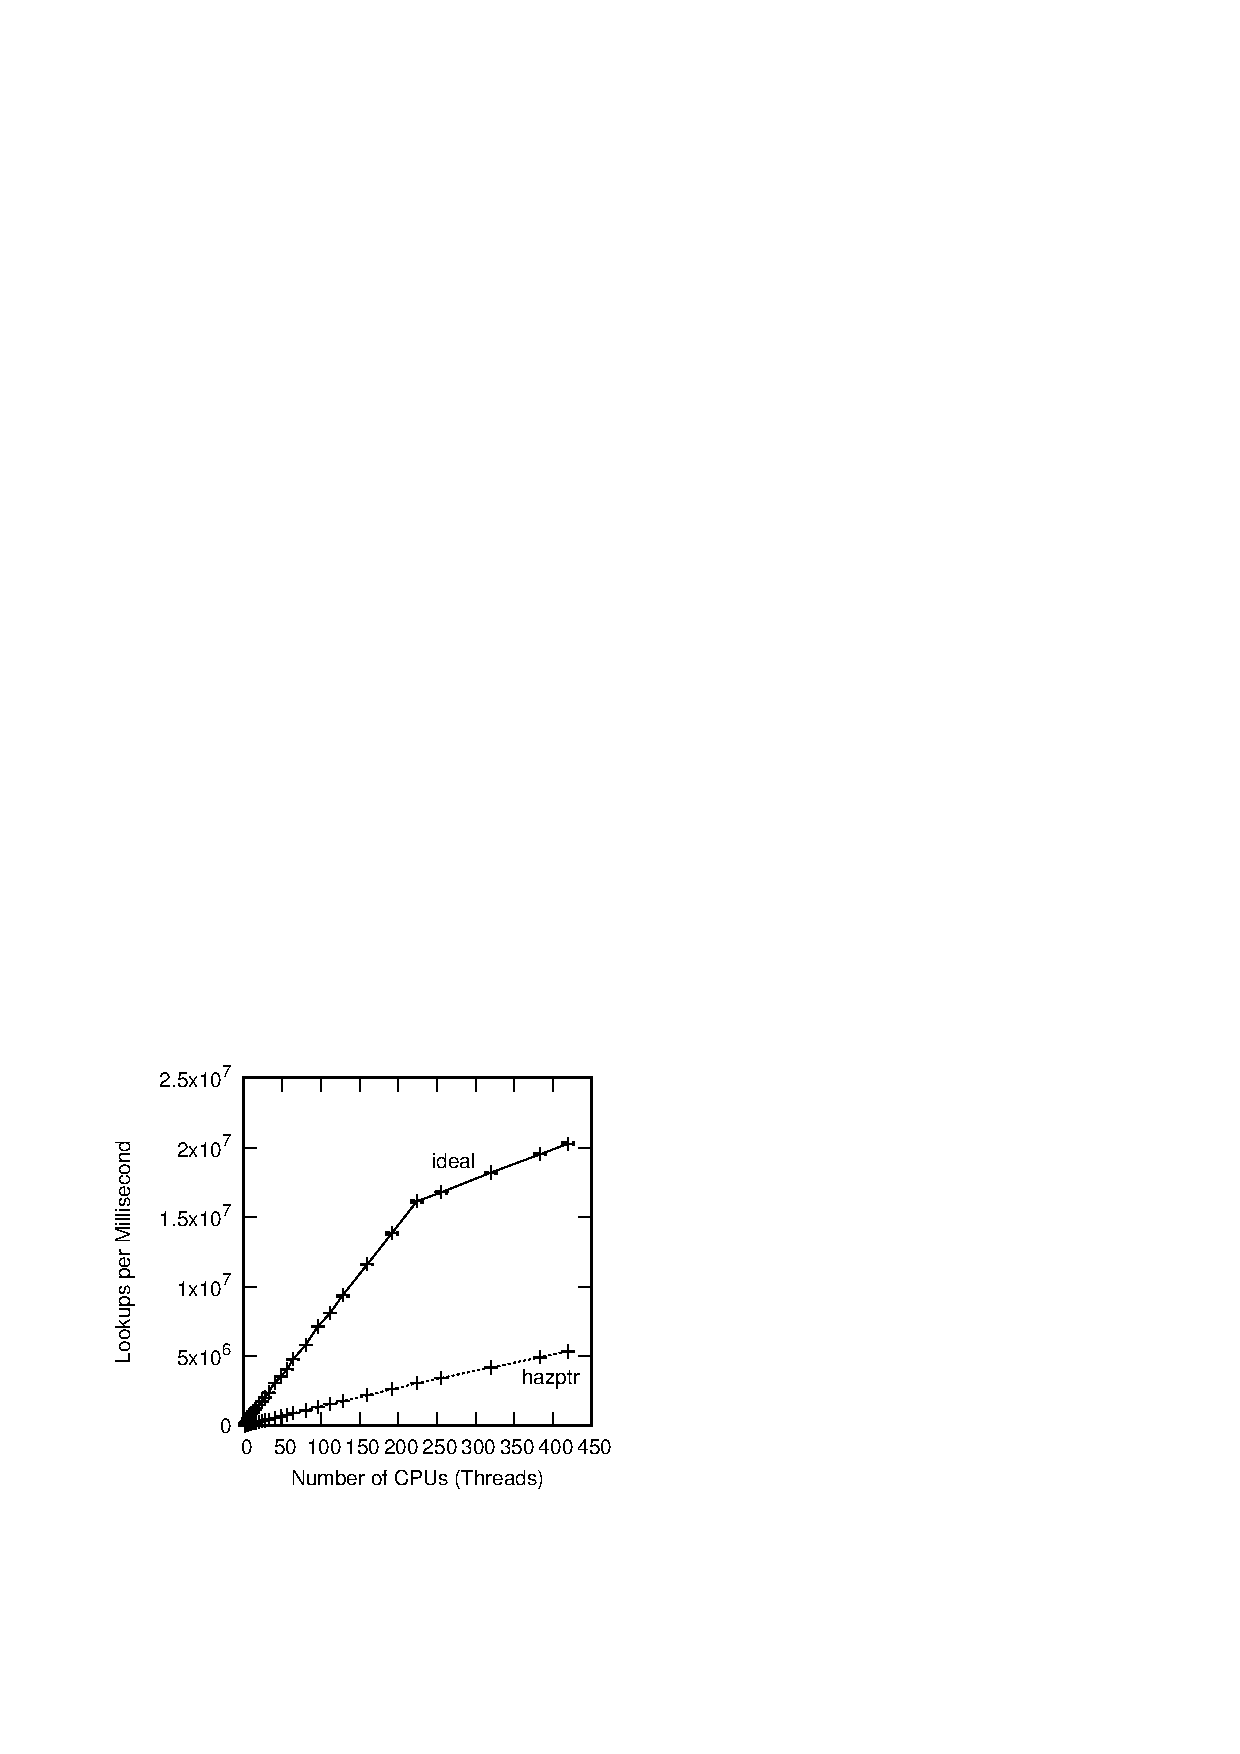
\includegraphics{CodeSamples/defer/perf-hazptr}}
\caption{Pre-BSD Routing Table Protected by Hazard Pointers}
\label{fig:defer:Pre-BSD Routing Table Protected by Hazard Pointers}
\end{figure}

Figure~\ref{fig:defer:Pre-BSD Routing Table Protected by Hazard Pointers} 는
해저드 포인터로 보호되는 Pre-BSD 라우팅 알고리즘의
Figure~\ref{fig:defer:Pre-BSD Routing Table Protected by Reference Counting}
에서와 동일한 read-only 워크로드에서의 성능을 보입니다.
해저드 포인터가 레퍼런스 카운팅에 비해 훨씬 잘 확장되긴 하지만, 해저드 포인터는
여전히 읽기 쓰레드가 공유 메모리에 쓰기를 할 것을 필요로 하며 (대신 훨씬 개선된
레퍼런스의 로컬리티를 제공합니다), 각 오브젝트 방문마다 메모리 배리어와 재시도
여부 검사를 필요로 합니다.
그로 인해 해저드 포인터의 성능은 이상적인 것에 비하면 훨씬 떨어집니다.
반면에, 동시의 레퍼런스 카운팅으로의 순진한 접근법들과 달리, 해저드 포인터는
동시의 업데이트가 섞인 워크로드에도 정확히 동작합니다.
다른 메커니즘들과의 추가적인 성능 비교는
Chapter~\ref{chp:Data Structures} 와 다른
출간물들~\cite{ThomasEHart2007a,McKenney:2013:SDS:2483852.2483867,MagedMichael04a}
에서 찾을 수 있습니다
\iffalse

Figure~\ref{fig:defer:Pre-BSD Routing Table Protected by Hazard Pointers}
shows the hazard-pointers-protected Pre-BSD routing algorithm's
performance on the same read-only workload as for
Figure~\ref{fig:defer:Pre-BSD Routing Table Protected by Reference Counting}.
Although hazard pointers scales much better than does reference counting,
hazard pointers still require readers to do writes to shared
memory (albeit with much improved locality of reference),
and also require a full memory barrier and retry check for each
object traversed.
Therefore, hazard pointers's performance is far short of ideal.
On the other hand, unlike naive approaches to concurrent reference-counting,
hazard pointers do operate correctly for workloads
involving concurrent updates.
Additional performance comparisons with other mechanisms may be found in
Chapter~\ref{chp:Data Structures}
and in other publications~\cite{ThomasEHart2007a,McKenney:2013:SDS:2483852.2483867,MagedMichael04a}.
\fi

\QuickQuiz{}
	논문 ``Structured Deferral: Synchronization via
	Procrastination''~\cite{McKenney:2013:SDS:2483852.2483867} 은 해저드
	포인터가 이상적인 경우에 가까운 성능을 보인다는 걸 보였습니다.
	Figure~\ref{fig:defer:Pre-BSD Routing Table Protected by Hazard Pointers}
	에선 무슨 일이 일어난거죠???
	\iffalse

	The paper ``Structured Deferral: Synchronization via
	Procrastination''~\cite{McKenney:2013:SDS:2483852.2483867}
	shows that hazard pointers have near-ideal performance.
	Whatever happened in
	Figure~\ref{fig:defer:Pre-BSD Routing Table Protected by Hazard Pointers}???
	\fi
\QuickQuizAnswer{
	첫째로,
	Figure~\ref{fig:defer:Pre-BSD Routing Table Protected by Hazard Pointers}
	는 1차원적 y-축을 갖는데 반해 ``Structured Deferral'' 논문에서의
	그래프는 로그스케일 y-축을 갖습니다.
	다음으로, 그 논문은 가벼운 일을 하는 해시 테이블을 사용했고,
	Figure~\ref{fig:defer:Pre-BSD Routing Table Protected by Hazard Pointers}
	의 수행은 10개 원소의 간단한 링크드 리스트를 사용했는데, 이는, 해저드
	포인터가 이 워크로드에서 ``Structured Deferral'' 논문에서의 것보다 더
	큰 메모리 배리어 페널티를 받았다는 뜻입니다.
	마지막으로, 그 논문은 더 커다랗고 오래된 x86 시스템을 쓴 반면,
	Figure~\ref{fig:defer:Pre-BSD Routing Table Protected by Hazard Pointers}
	의 결과를 만드는데 사용된 시스템은 더 신형이고 더 작은
	시스템이었습니다.
	\iffalse

	First,
	Figure~\ref{fig:defer:Pre-BSD Routing Table Protected by Hazard Pointers}
	has a linear y-axis, while most of the graphs in the
	``Structured Deferral'' paper have logscale y-axes.
	Next, that paper uses lightly-loaded hash tables, while
	Figure~\ref{fig:defer:Pre-BSD Routing Table Protected by Hazard Pointers}'s
	uses a 10-element simple linked list, which means that hazard pointers
	face a larger memory-barrier penalty in this workload than in
	that of the ``Structured Deferral'' paper.
	Finally, that paper used a larger and older x86 system, while
	a newer but smaller system was used to generate the data
	shown in
	Figure~\ref{fig:defer:Pre-BSD Routing Table Protected by Hazard Pointers}.
	\fi

	또한, 비대칭적 배리어 쌍의 사용~\cite{Windows2008FlushProcessWriteBuffers,JonathanCorbet2010sys-membarrier,Linuxmanpage2018sys-membarrier}
	이 가능한 시스템에서는 읽기 쪽 해저드 포인터 메모리 배리어를 없애기
	위해 사용될 것이
	제안되었는데~\cite{DavidGoldblatt2018asymmetricFences}, 이렇게 되면
	해저드 포인터의 성능을 이 그림에서 보인 것보다 더 향상시킬 수 있을
	겁니다.
	\iffalse

	In addition, use of pairwise asymmetric
	barriers~\cite{Windows2008FlushProcessWriteBuffers,JonathanCorbet2010sys-membarrier,Linuxmanpage2018sys-membarrier}
	has been proposed to eliminate the read-side hazard-pointer
	memory barriers on systems supporting this notion~\cite{DavidGoldblatt2018asymmetricFences},
	which might improve the performance of hazard pointers beyond
	what is shown in the figure.
	\fi

	항상 그렇듯, 비용은 경우에 따라 다를 수 있습니다.
	이 성능의 차이를 놓고 보면, 해저드 포인터가 (메모리 배리어 오버헤드가
	최소한 캐시 미스 페널티와 겹칠만큼) 매우 커다란 데이터 구조체에서나
	해시 테이블과 같이 탐색 작업이 최소한의 해저드 포인터만을 필요로 하는
	경우에는 가장 이상적인 성능을 줄 것임이 분명합니다.
	\iffalse

	As always, your mileage may vary.
	Given the difference in performance, it is clear that hazard
	pointers give you the most ideal performance either for
	very large data structures (where the memory-barrier overhead
	will at least partially overlap cache-miss penalties) and
	for data structures such as hash tables where a lookup
	operation needs a minimal number of hazard pointers.
	\fi
} \QuickQuizEnd

다음 섹션은 해저드 포인터에서 더 개선을 하기 위해서 read-side 에서의 쓰기도
오브젝트별 메모리 배리어도 없애주는 시퀀스 락을 사용해 보겠습니다.
\iffalse

The next section attempts to improve on hazard pointers by using
sequence locks, which avoid both read-side writes and per-object memory
barriers.
\fi
